\section{A probability sort for continuous model theory}
\label{sec:probability-models}

The repository already develops finite-net semantics for fixed continuous
formulas~\cite{repo-recent}.  Here is a new client of that interface: an
entire sort of probability distributions, constructed from finite transport
and explicit nets.  Its outputs are genuine finitely supported probability
laws.  Quantifiers over that sort can express optimization of several
expectations at once.  No compactness theorem for arbitrary theories, or
general construction of a measure from its moments, is needed.

\subsection{Exact finite transport without an unbounded optimization oracle}

Fix a nonempty PR-presented rational metric space \(X\), a supplied rational
diameter bound \(D\geq0\), and a fixed PR provider of nonempty finite
\(\delta\)-nets at every requested dyadic radius.  An atomic probability code is
\[
 \mu=\sum_{i<p}a_i\delta_{x_i},\qquad
 a_i\in\mathbb Q_{\geq0},\quad \sum_{i<p}a_i=1,
\]
where \(\delta_x\) denotes unit mass at \(x\).  Repeated support points
and zero weights are harmless.  For another such code
\(\nu=\sum_{j<q}b_j\delta_{y_j}\), a coupling is a rational matrix
\(\pi_{ij}\geq0\) with row sums \(a_i\) and column sums \(b_j\).
Its cost is \(\sum_{i,j}\pi_{ij}d(x_i,y_j)\).

\begin{lemma}[Bounded exact transport]\label{lem:transport-forest}
The minimum coupling cost is rational and primitive recursive in the
atomic codes and the fixed PR distance recipe.  It can be computed by
enumerating at most \(2^{pq}\) edge subsets of the bipartite support graph,
retaining feasible forests, and taking the least of their costs.
\end{lemma}
\begin{proof}
For a proposed forest, a leaf has just one incident edge.  The remaining
marginal at that leaf therefore determines the edge weight.  Subtract it
from its neighbor's remaining marginal, set the leaf marginal to zero,
and remove the edge.  Reject a negative weight, a negative remaining
marginal, or an isolated vertex with a nonzero remaining marginal.
After at most \(pq\) eliminations, accept exactly when all residual
marginals are zero.  This constructs the unique feasible matrix supported
on the proposed forest, if one exists; zero assigned edges may remain in
the originally proposed support.

It remains to prove that this finite list contains an optimizer.  Start
from any feasible coupling, for example \(\pi_{ij}=a_ib_j\).  If its
positive-support graph has a cycle, alternate plus and minus signs around
that cycle.  The cycle is even.  Choose the orientation for which the
signed sum of edge costs is nonpositive; this is a rational comparison.
Let \(t>0\) be the least weight on its minus edges.  Add \(t\) on the
plus edges and subtract it on the minus edges.  Every row and column sum
is unchanged, all entries remain nonnegative, cost does not increase,
and at least one positive edge disappears.  No edge outside the previous
positive support is introduced.  After at most \(pq\) such steps the
support is a forest.

Thus every rational feasible coupling has a feasible forest coupling of
no greater cost.  At least one exists, and the least cost in the finite
forest list is no larger than that of any feasible coupling.  The list
therefore supplies an actual minimum.  Cycle search, minimum selection,
leaf elimination, rational arithmetic and all loop bounds are finite PR
operations; their correctness invariants are the marginal equations,
nonnegativity, the cost inequality and the decreasing support size.
\end{proof}

For ordinary classical semantics, the same finite cycle elimination applies
to a real feasible matrix.  On the final forest its weights are determined
by leaf subtraction from rational marginals, hence are rational.  Thus the
computed minimum also equals the usual finite real transport optimum.
The arithmetic algorithm itself processes rational matrices only.

Write this minimum as \(W_1(\mu,\nu)\), the usual transport-cost construction~\cite{peyre2019}.  The enumerator is a completeness
baseline, not a polynomial-time implementation.  A faster producer can
submit a feasible coupling and rational numbers \(\alpha_i,\beta_j\)
such that
\[
 \alpha_i+\beta_j\leq d(x_i,y_j),\qquad
 \sum_{i,j}\pi_{ij}d(x_i,y_j)=\sum_i a_i\alpha_i+\sum_j b_j\beta_j.
\]
For every feasible coupling, summing the first inequalities proves that
its cost is at least the displayed right side.  Equality therefore
certifies optimality using only finite arithmetic.  Existence of such
potentials is not needed by the bounded forest algorithm.

\begin{lemma}[Transport pseudometric and expectation stability]
\label{lem:transport-metric}
The function \(W_1\) is a rational pseudometric on atomic codes, of
diameter at most \(D\).  If a fixed function \(f\) is \(L\)-Lipschitz,
then
\[
 \left|\sum_i a_if(x_i)-\sum_j b_jf(y_j)\right|
       \leq L W_1(\mu,\nu).
\]
The same finite estimate applies to computable rational enclosures of
\(f\), with their evaluation errors added separately.
\end{lemma}
\begin{proof}
Nonnegativity is immediate.  A diagonal coupling has zero self-cost;
transposition proves symmetry.  For the triangle inequality, take
couplings \(\pi_{ij}\) between \(\mu,\nu\) and \(\sigma_{jk}\)
between \(\nu,\lambda\), and set
\[
 \gamma_{ijk}=
 \begin{cases}
 \pi_{ij}\sigma_{jk}/b_j,&b_j>0,\\
 0,&b_j=0.
 \end{cases}
\]
When \(b_j=0\), nonnegativity and the marginal equations force every
incident entry of both matrices to vanish.  Consequently
\(\theta_{ik}=\sum_j\gamma_{ijk}\) has the required marginals.
Multiply \(d(x_i,z_k)\leq d(x_i,y_j)+d(y_j,z_k)\) by
\(\gamma_{ijk}\) and sum.  Its cost is at most the sum of the two
input costs.  Taking their finite minimizers proves the triangle inequality.
Every coupling has total mass one and each ground distance is at most
\(D\), giving the diameter bound.  Finally, for any coupling,
\[
 \sum_i a_if(x_i)-\sum_j b_jf(y_j)
    =\sum_{i,j}\pi_{ij}\bigl(f(x_i)-f(y_j)\bigr).
\]
The triangle inequality and the Lipschitz bound give the stated estimate
at a minimizing coupling.  All divisions retain the explicitly tested
positive-marginal guard.
\end{proof}

\subsection{A finite net of actual probability laws}

\begin{theorem}[Explicit total boundedness]\label{thm:probability-net}
Let \(c_0,\ldots,c_{m-1}\) be a nonempty \(\delta\)-net of \(X\).
For any positive integer \(N\), all laws
\[
 \sum_{i<m}\frac{n_i}{N}\delta_{c_i},\qquad
 n_i\in\{0,\ldots,N\},\quad\sum_i n_i=N,
\]
form a \(\delta+D(m-1)/N\)-net of the atomic-law space.
There are at most \((N+1)^m\) candidates, each a valid probability law.
\end{theorem}
\begin{proof}
Move each point of the input support to the first center at distance at
most \(\delta\).  A bounded scan finds it.  The resulting center law
has weights \(p_i\), and the explicit deterministic coupling has cost at
most \(\delta\).  Put
\[
 n_i=\lfloor Np_i\rfloor\quad(i<m-1),\qquad
 n_{m-1}=N-\sum_{i<m-1}n_i,\qquad q_i=n_i/N.
\]
All \(q_i\) are nonnegative and sum to one.  For each early coordinate
let \(r_i=p_i-q_i\); then \(0\leq r_i<1/N\).  The last coordinate
has gained exactly \(s=\sum_{i<m-1}r_i\).  Keep common mass at its
center and transport the excess \(r_i\) from center \(i\) to the last
center.  This explicit coupling costs at most
\(Ds\leq D(m-1)/N\).  Equivalently, the total variation distance is
\(\frac12\sum_i|p_i-q_i|=s\).  Combine this with the first move by
the triangle inequality.  Enumerating all integer tuples in the stated
box and checking their sum produces the net.  For \(m=1\) the rounding
error is zero and any \(N\geq1\) works.
\end{proof}

For dyadic target radius \(\eps>0\), choose a base net at
\(\delta=\eps/2\) and
\[
 N=\max\left(1,\left\lceil\frac{2D(m-1)}{\eps}\right\rceil\right).
\]
This is a PR choice from positive rational data.  It avoids inferring a
covering-number bound from bare classical compactness.  Its possibly large
enumeration size is explicit; no polynomial dependence on dimension or
precision is claimed.
For an arbitrary positive rational target, first choose a dyadic base-net
radius at most \(\eps/2\) by bounded search; the same bound for \(N\)
then applies.

Apply the common completion interface to this atomic pseudometric.
For a regular name of laws and target \(\eps=2^{-k}\), take its
\((k+1)\)-st atomic approximant and use the dense atomic net at radius
\(\eps/2\).  The two losses are at most \(\eps/2\) each.  Thus the
represented Wasserstein completion has the finite nets required for a
compact probability sort in the quantitative semantics.  Completeness
here refers to supplied uniformly PR modulated families, as in
Section~\ref{sec:completion}; it is not an internal selection principle
for arbitrary sequences or arbitrary open covers.

Each fixed Lipschitz expectation extends by
Lemma~\ref{lem:transport-metric}.  If a standard probability measure is
given externally together with the required PR atomic approximations and
transport estimates, these expectations agree with its ordinary
integrals.  The construction does not assert that every classical measure
has such a presentation, nor construct an arbitrary measure from a
positive functional.  No Prokhorov theorem is used.

\subsection{Quantified continuous formulas over probability laws}

The supplied language may have the point sort \(X\), the probability
sort just constructed, their metrics, fixed Lipschitz observables, and
expectation atoms \(\mathbb E_\mu f\).  Ground data and their moduli
are fixed PR recipes.  Functions with real values are evaluated with
supplied rational enclosures.  Use \(\min,\max,|\cdot|\), rational
affine combinations, and \(\inf,\sup\) quantifiers.  If the
\([0,1]\)-valued convention of continuous logic is desired, retain
range bounds and clip the appropriate connectives to that interval.
There is no quantification over all predicates or all probability measures
as an internal higher-order object.

Every fixed formula receives a Lipschitz vector for its free variables.
For absolute value retain the input vector; for minimum or maximum take
the componentwise maximum of the two vectors; for an affine combination
\(\sum_j a_j\varphi_j+c\), use
\(\sum_j|a_j|L(\varphi_j)\).  Quantifying a variable preserves the
remaining coordinate bounds.  For example, a fixed \(F(x,z)\) that is
\(L_x\)-Lipschitz in \(x\) and \(L_z\)-Lipschitz in \(z\) gives
\[
 |\mathbb E_\mu F(x,z)-\mathbb E_\nu F(y,z)|
 \leq L_xd(x,y)+L_zW_1(\mu,\nu).
\]
Split the difference by keeping \(\mu\) fixed in the first term;
finite averaging proves that term's bound, and the coupling estimate
proves the second.

\begin{proposition}[Finite quantifier evaluation]\label{prop:probability-formula}
For a fixed formula with the supplied atomic evaluators and Lipschitz
data, every requested truth-value precision has a PR finite evaluator.
At a quantifier over a sort with an \(r\)-net, replacing its infimum
or supremum by the finite minimum or maximum loses at most \(Lr\),
where \(L\) is the bound for that variable.  If every entry is evaluated
within \(\eta\), the total loss at that node is at most \(Lr+\eta\).
\end{proposition}
\begin{proof}
For an infimum, every net point belongs to the sort, while every point
is within \(r\) of a net point whose formula value differs by at most
\(Lr\).  These two inequalities bound the finite minimum on either
side of the infimum.  A uniform perturbation of every table entry by
\(\eta\) perturbs its minimum by at most \(\eta\): compare each
table at an index minimizing the other.  Negation gives the supremum
case.  Absolute value, minimum and maximum are nonexpansive; the affine
error bound is \(\sum_j|a_j|\eta_j\).  External induction on the
fixed formula therefore supplies an explicit error recurrence.  Choose
net radii and work precisions from these bounds, and evaluate the finite
tables by bounded loops.  Fixed formula depth and the supplied PR
covering bounds make the whole evaluator PR.  In a purely represented
construction the successive finite values themselves define the scalar
truth-value name; the same inequalities prove coherence, so no exact
infimum-existence oracle is being used.
\end{proof}

Several occurrences of one expectation can share its computed finite sum
and its error certificate.  The reverse-weight verifier of
Section~\ref{sec:budgets} combines evaluator and quantifier-net errors.
This is an application of the earlier semantics, with a newly constructed
probability sort and actual finite distribution witnesses.  It provides
neither general model existence nor a completeness theorem for arbitrary
continuous theories.

\subsection{An exact quantified example and its proof}

Take the rational dense interval \(X=[0,1]\cap\mathbb Q\), with
\(d(x,y)=|x-y|\) and dyadic grid nets.  The observables \(x\) and
\(x^2\) have Lipschitz bounds \(1\) and \(2\), since
\(|x^2-y^2|=|x-y|(x+y)\leq2|x-y|\).  In the represented probability
sort, the following truth value is exact:
\begin{equation}\label{eq:probability-moment-example}
 \inf_\mu\max\left(
     \left|\mathbb E_\mu x-\frac12\right|,
     \left|\mathbb E_\mu x^2-\frac34\right|
                       \right)=\frac18.
\end{equation}
Indeed \(0\leq x^2\leq x\) on the interval, so finite positivity
and completion give \(m_2\leq m_1\) for the two moments.  If the
displayed maximum is \(t\), then
\[
 \frac34-t\leq m_2\leq m_1\leq\frac12+t,
 \qquad\text{hence}\qquad t\geq\frac18.
\]
The genuine probability law
\(\mu=(3/8)\delta_0+(5/8)\delta_1\) has
\(m_1=m_2=5/8\), so its two errors are both \(1/8\).
It attains the bound.  This proves the quantified equality and exhibits
its witness without an appeal to abstract attainment or model existence.
For the arithmetic route, first prove the lower bound for an atomic law
by the displayed finite inequalities.  The objective is
\(2\)-Lipschitz in \(W_1\), so approximation and rational slack removal
pass that lower bound to every represented law; the upper bound already
has the explicit atomic witness.
The argument also shows why two moment targets cannot be treated as
independent real parameters: their common probability law forces an
inequality between them.

The feasible moment region in Figure~\ref{fig:observations} has a short
finite proof. Positivity of the square gives
$m_2-m_1^2=\mathbb E(x-m_1)^2\ge0$, while $x^2\le x$ gives
$m_2\le m_1$. Conversely, a rational pair $0<m\le1$, $m^2\le v\le m$
is attained by placing mass $m^2/v$ at $v/m$ and the remaining mass at zero.
Both masses are nonnegative, the support lies in $[0,1]$, and direct
calculation gives moments $(m,v)$. The case $m=0$ forces $v=0$ and uses
$\delta_0$. Thus the figure is derived from these exact inequalities and
witnesses, not from sampled numerical optimization.

\begin{figure}[tbp]
\centering
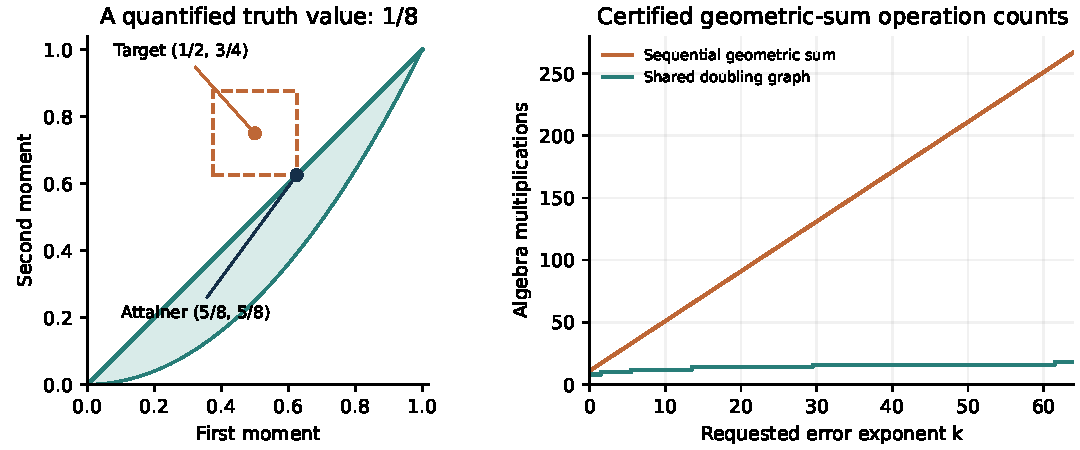
\includegraphics[width=\textwidth]{figures/observations.pdf}
\caption{Left: moment constraints make the continuous optimization problem
concrete. The smallest square centered at the target that meets the feasible
region has radius $1/8$. Right: algebra-operation counts for the explicit
Neumann clock $q=3/4$, $s=4$, $N=4(k+3)$, compared with its doubling evaluator.
These are exact operation counts for the prescribed algorithms, not elapsed-time
or bit-complexity benchmarks.}\label{fig:observations}
\end{figure}

\subsection{Formalization boundary and exact artifacts}

Define \code{AtomicLawCode} by a finite support array and rational weights
with Boolean nonnegativity and mass-one checks.  Define
\code{CouplingCode} by a rectangular rational array and its marginal
checks.  Implement \code{forestSolve}, \code{transport},
\code{pushRound}, and \code{probabilityNet} by the displayed bounded
algorithms.  Prove leaf-elimination preservation, cycle elimination,
finite gluing with the zero-marginal case, the rounding coupling, and
expectation stability in that order.  These are the additional finite
obligations before applying the already stated completion interface.
For object iPRA, each loop invariant consists of finite Boolean conditions,
cross-multiplied marginal equalities, and rational cost inequalities.
No unrestricted real quantifier is used as an induction matrix.

The checked Lean \code{argminQ_optimal} and
\code{finite_minimum_stability} kernels supply the finite quantifier
step.  The exact/supersolution budget theorem supplies shared error
propagation.  The transport and probability-net constructions themselves
are human proofs plus an implementation outline here, not completed Lean
theorems.  The accompanying \code{code/probability_models.py} uses exact
rational arithmetic to enumerate forests, check primal/dual certificates,
exercise gluing with a zero middle mass, construct a finite law net and
reproduce \eqref{eq:probability-moment-example}.  It records a denominator-8
three-center net with 45 valid laws and the exact attaining endpoint law.
These are finite implementation checks, not a substitute for the
object-theory derivations or a general construction of probability measures.
